\documentclass[12pt]{article}
\usepackage[utf8]{inputenc}
\usepackage[dutch]{babel}
\usepackage[rightcaption]{sidecap}
% \usepackage{minted}
\usepackage{graphicx}
\usepackage[colorlinks=true, allcolors=blue]{hyperref}
\usepackage{sectsty}
\usepackage[paperheight=29.7cm,paperwidth=21cm,textwidth=15cm]{geometry} %A4 size
\usepackage{fancyhdr}
\usepackage[siunitx]{circuitikz}
\usepackage{tabularx}
\usepackage{physunits}
\usepackage{booktabs}
\usepackage{tikz}
\usepackage{pgfplots}

\usepackage[nocompress]{cite}
\usepackage{cite}


\usepackage{parskip}
\usepackage{amsmath,amssymb,amsfonts}
\usepackage{algorithmic}

% The preceding line is only needed to identify funding in the first footnote. If that is unneeded, please comment it out.
\usepackage{textcomp}
 % More defined colors
% We will externalize the figures



% Footers/Headers opmaak:
\pagestyle{fancy}
\lhead{}
\chead{\textit{Practicum 1: Digitale Techniek - Logische poorten 
}}
\rhead{}
\lfoot{\textit{Semih Can Karakoç}}
\cfoot{\textit{\today}}
\rfoot{\textit{\thepage}}
\renewcommand{\headrulewidth}{0.1pt}
\renewcommand{\footrulewidth}{0.4pt}

% Afbeelding settings:
\graphicspath{ {./Figures/} }
% \sectionfont{\left}
% \subsectionfont{\centering}
% \subsubsectionfont{\centering}

% Voorpagina opmaak:
\title{\textbf{Practicum 1. Logische poorten}}
\author{\textit{Semih Can Karakoç (695258)}}
\date{\textit{\today}}

% Begin document
\begin{document}

\clearpage\maketitle    % Pas opmaak toe aan voorpagina
\thispagestyle{empty}  % Haal page number weg
% Voorpagina plaatje:
\begin{figure}[h]
    \centering
    % \includegraphics[width=0.6\textwidth]{ELEKTRA.png}
\end{figure}
\pagebreak

\tableofcontents    % Inhoudsopgave
\pagebreak

\section{Inleiding}
In dit practicum is onderzocht naar de werking van RC-schakelingen. 
Het doel is om verschillende aspecten van deze schakelingen te begrijpen en te kunnen berekenen, zoals de RC-tijdconstante, de kantelfrequentie en de overdracht van een RC filter.
Daarvoor zijn er drie experimenten uitgevoerd en zijn de bijbehorende meetgegevens verzameld en verwerkt in dit verslag. 
Deze gegevens zullen we vervolgens interpreteren, met als doel om tot een goed begrip van de werking van RC schakelingen te komen. 
Het verslag zal eerst de theorie behandelen en daarna ingaan op de bijbehorende opdrachten, de onderzoeksvragen en tenslotte eindigen met een conclusie.
\pagebreak
\section{Probleem- en doelstelling}
Dit verslag bevat twee onderzoeksvragen, namelijk:
\begin{enumerate}
    \item \textit{``Hoe berekenen we de tijdconstante van een RC schakeling?''};
    \item \textit{``Hoe berekenen we de kantelfrequentie en de overdracht van een RC filter?''}. 
\end{enumerate}
\vspace{0,5cm}
De volgende doelstellingen die horen bij dit practicum zijn:
\begin{enumerate}
    \item Inzicht te verkrijgen in logische functies die ten grondslag liggen aan de digitale techniek;
    \item waarnemingen te verrichten aan de bijbehorende eenvoudige logische schakelingen;
    \item de bijbehorende meetgegevens en waarheidstabellen op een juiste wijze te verkrijgen en te interpreteren;
    \item de vergaarde gegevens te verwerken tot een verslag.
\end{enumerate}

\vspace{0,5cm}
Aan het einde van dit verslag onder het kopje \ref{Conclusie}:\textit{``Conclusie''} zal de probleemstelling beantwoord worden!
\pagebreak

\section{Benodigdheden}
Hieronder zijn de benodigdheden benoemd die essentieel zijn voor tijdens het practicum:
\begin{enumerate}
    \item Een oscilloscoop: een oscilloscoop is een apparaat dat gebruikt wordt om elektrische signalen te meten en weer te geven op een scherm. Hiermee kun je de vorm, de frequentie en de amplitude van het signaal bepalen \cite{Fluke_oscilloscope};
    \item Twee meetprobes: meetprobes zijn soort verleng/aansluitdraden die gebruikt worden om elektrische signalen op te nemen en/of te versterken. Ze worden aangesloten op de oscilloscoop om signalen op te nemen en te analyseren \cite{Fluke_probes};
    \item Een patroongenerator: een patroongenerator is een instrument dat elektrische signalen kan genereren met behulp van vooraf ingestelde parameters, zoals de frequentie, de amplitude en de faserelatie. Met een patroongenerator kun je verschillende soorten signalen genereren om je experimenten mee uit te voeren \cite{witte2002electronic};
    \item Een DC spanningsbron: een DC spanningsbron is een apparaat dat constante elektrische spanning levert, zoals een batterij of een voeding. De DC spanningsbron wordt gebruikt om de RC schakelingen mee te voeden \cite{Boylestad_1997, patgenwp};
    \item Een breadboard: een breadboard is een apparaat waarop elektronische componenten op een eenvoudige manier met elkaar verbonden kunnen worden zonder dat ze permanent op een printplaat hoeven te worden gesoldeerd \cite{buckley2022whatisabreadboard};
    \item Een aantal snoeren: snoeren worden gebruikt om de componenten op het breadboard met elkaar te verbinden;
    \item Een weerstand: een weerstand is een component dat elektrische stroom beperkt. De weerstand wordt gebruikt om de stroomsterkte in een circuit te reguleren of om spanning te verdelen over verschillende componenten \cite{Schagrin1963};
    \item Een condensator: een condensator is een component dat elektrische lading kan opslaan. De condensator wordt gebruikt om tijdelijk elektrische lading op te slaan en af te geven wanneer dat nodig is. In dit practicum gebruiken we de condensator om RC schakelingen mee te bouwen \cite{bird2010electrical};
\end{enumerate}
\pagebreak

\section{Theoretisch kader}
lol

\pagebreak
\section{Methode}
lol

\pagebreak
\section{Opdracht 1: de 7404}
In de eerste opdracht zijn de volgende deelvragen onderzocht en beantwoord, namelijk:
\begin{enumerate}
    \item Bepaal aan de hand van de datasheet welke type poort dit IC bevat?
    \item Tot welke logica familie behoort dit type IC?
    \item Hoeveel poorten bevat dit IC?
    \item Sluit met behulp van de datasheet het IC op correcte wijze aan op het IC board;
    \item Ga de werking van de poort na;
    \item Stel de bijbehorende waarheidstabel op;
    \item Op het digiboard zelf ontbreekt de poort die wij onderzoeken. Welke poort(en) van het digiboard kunnen eventueel als alternatief worden gebruikt?
    \item Teken de bijbehorende logische schakeling;
    \item Ga de werking van deze alternatieve poort na en concludeer of de werking hetzelfde is. 
\end{enumerate} 

\begin{figure}[h]
    \centering
    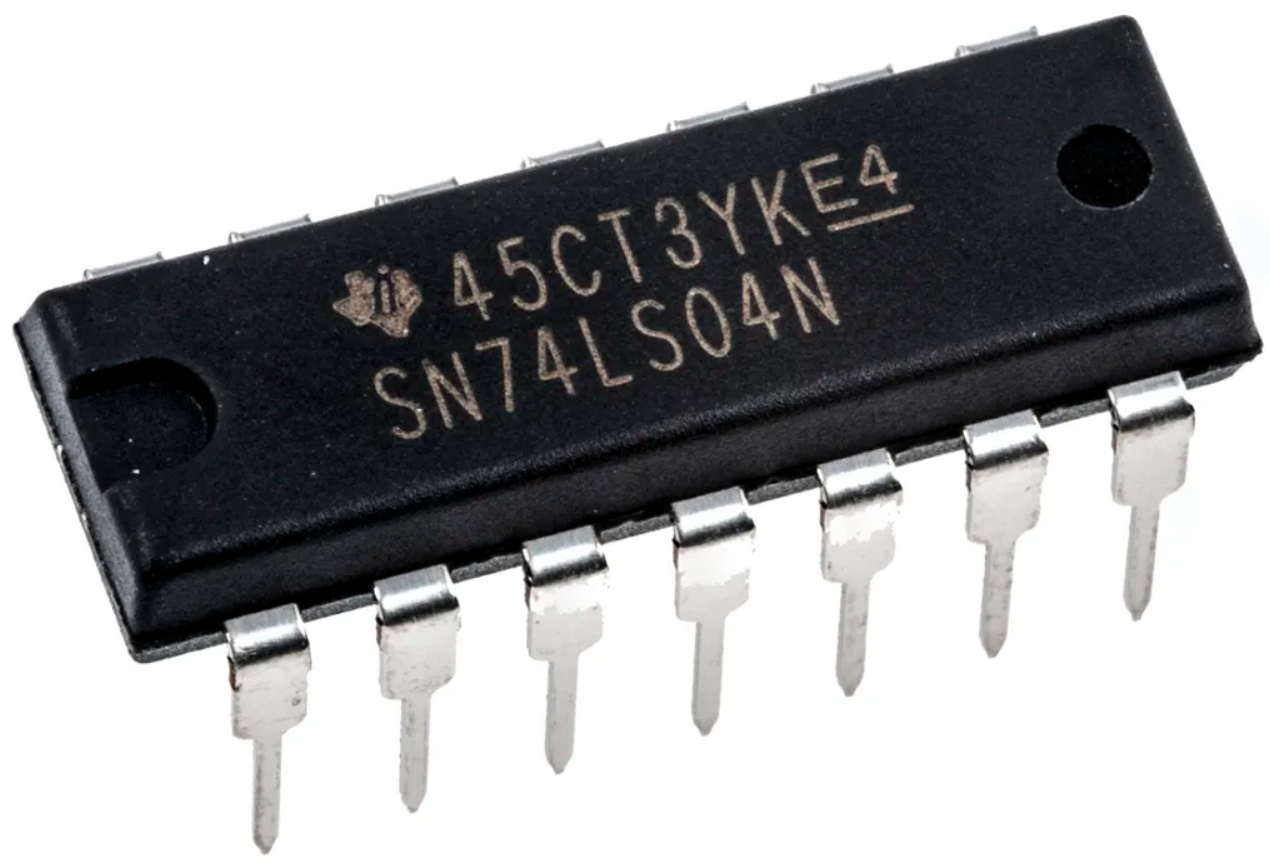
\includegraphics[width=0.5\textwidth]{7404_PLAATJE.png}
    \caption{Foto van de 7404 IC.}
    \label{fig:7404}
\end{figure}

\pagebreak
\subsection{Bepaal aan de hand van de datasheet welke type poort dit IC bevat}
Volgens de datasheet van de 7404 IC, bevat deze IC in totaal zes NOT-poorten (inverters).

\subsection{Tot welke logica familie behoort dit type IC}
Deze IC behoort tot de Transistor-Transistor-Logica (TTL) familie. Dit is te herkennen aan de 7400 serie nummering van de IC. 

\subsection{Hoeveel poorten bevat dit IC}
Volgens de datasheet van de 7404 bevat dit IC in totaal zes NOT-poorten, waarvan er zowel zes input-pennen als output-pennen aanwezig zijn.

\subsection{Sluit met behulp van de datasheet het IC op correcte wijze aan op het IC board}
Volgens de datasheet zijn:
\begin{enumerate}
    \item ``1, 3, 5, 9, 11, 13" de ingangspinnen;
    \item ``2, 4, 6, 8, 10, 12" de uitgangspinnen;
    \item ``7" de $GND$ pin;
    \item ``14" de $V_{cc}$ pin. 
\end{enumerate}

\subsection{De werking van de poort}
De werking van de NOT-poort in de 7404 IC is als volgt: \\
Als de input signaal HOOG (1) is, dan gaat de output signaal naar LAAG (0).\\ 
Als de input signaal LAAG (0) is, dan gaat de output signaal naar HOOG (1).

\subsection{De bijbehorende waarheidstabel}
\begin{displaymath}
    \begin{array}{|c||c|}
    Input (A) & Output (Q)\\ % Use & to separate the columns
    \hline % Put a horizontal line between the table header and the rest.
    1 & 0\\
    0 & 1\\
    \end{array}
    \end{displaymath}
\pagebreak

\subsection{Alternatieve poorten}
Als alternatief voor de NOT poort kunnen we ook een NAND poort of een NOR poort gebruiken.

\begin{figure}[h]
    \centering
    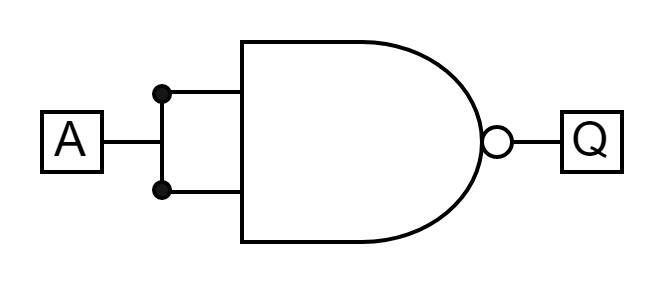
\includegraphics[width=0.5\textwidth]{NAND-NOT.png}
    \caption{Een alternatieve manier om een NOT poort te maken door middel van een NAND poort.}
    \label{fig:NANDNOT}
\end{figure}

\begin{figure}[h]
    \centering
    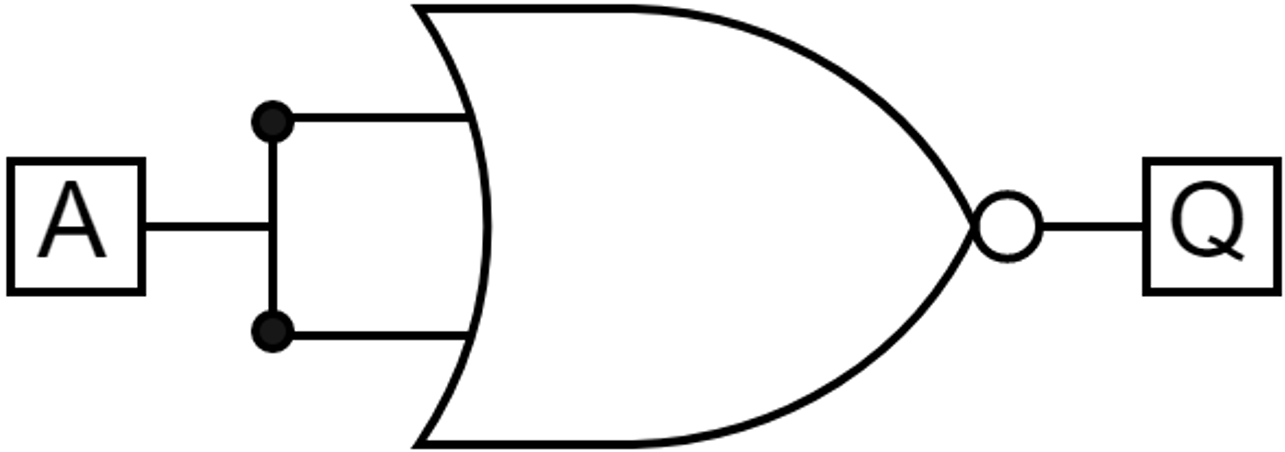
\includegraphics[width=0.45\textwidth]{NOR-NOT.png}
    \caption{Een alternatieve manier om een NOT poort te maken door middel van een NOR poort.}
    \label{fig:NORNOT}
\end{figure}
Zie hier onder de waarheidstabel van zowel de NAND als die van de NOR poort als bewijs dat beide poorten als een NOT poort gebruikt kunnen worden.
\begin{displaymath}
    \begin{array}{|c|c||c|c|}
    X & Y & NAND (\lnot()) & NOR (\lnot\lor)\\
    \hline 
    1 & 1 & 0 & 0\\
    0 & 0 & 1 & 1\\
    \end{array}
    \end{displaymath}

\subsection{De getekende logische schakeling}
\begin{figure}[h]
    \centering
    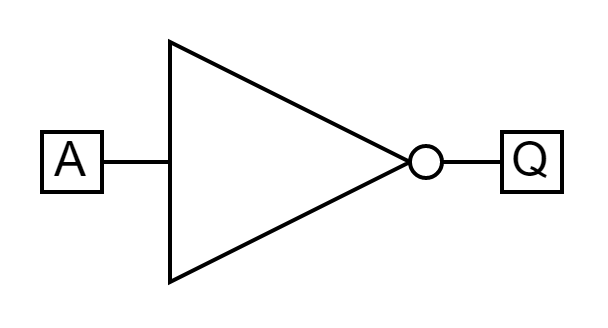
\includegraphics[width=0.3\textwidth]{INV.png}
    \caption{Getekende logische schakeling van de inverter (NOT poort).}
    \label{fig:INV}
\end{figure}

\begin{figure}[h]
    \centering
    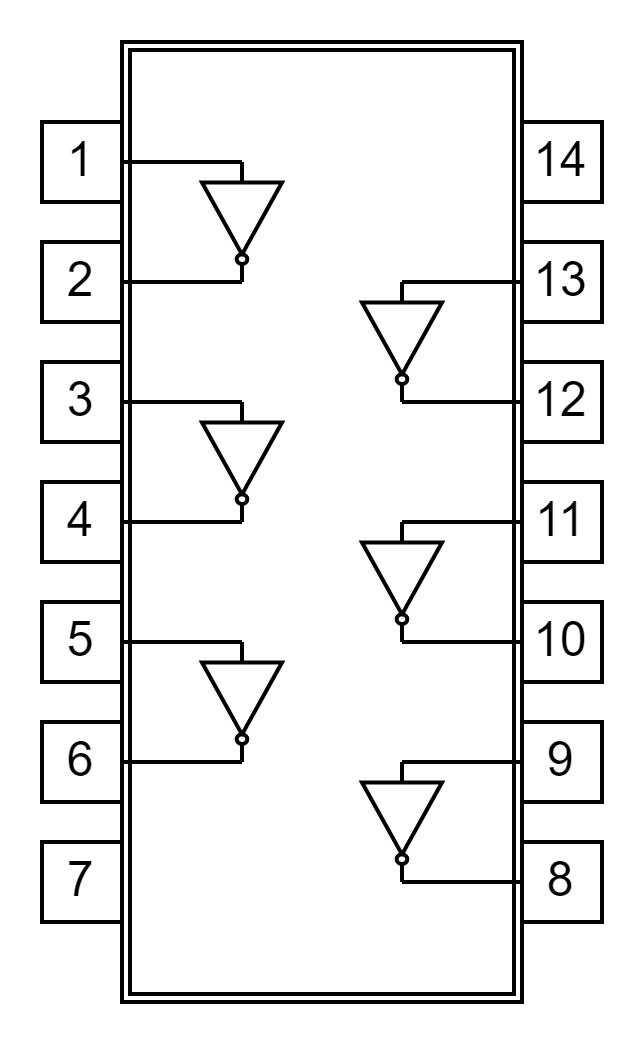
\includegraphics[width=0.3\textwidth]{7404_SCHEMA.png}
    \caption{Getekende logische schakeling van de 7404 IC. Hierbij is pin-14 de $V_{cc}$ aansluiting en is pin-7 de $GND$ aansluiting.}
    \label{fig:7404SCHEMA}
\end{figure}

\subsection{Ga de werking van deze alternatieve poort na en concludeer of de werking hetzelfde is}
De werking van de alternatieve poort moet semantisch equivalent zijn aan die van de NOT poort (inverter). 
Om te kunnen bewijzen dat beide logische poorten semantisch equivalent zijn moeten we de bijbehorende waarheidstabellen maken. De eerste waarheidstabel is die van de NOT poort (inverter).
\begin{displaymath}
    \begin{array}{|c||c|}
    A & \lnot A\\ % Use & to separate the columns
    \hline % Put a horizontal line between the table header and the rest.
    1 & 0\\
    0 & 1\\
    \end{array}
    \end{displaymath}
Wel is het belangrijk dat bij de NAND poort dat input X en Y altijd dezelfde waarde moeten hebben, dus als $X=1$ dan is $Y=1$, en als $X=0$ dan is $Y=0$.
\begin{displaymath}
    \begin{array}{|c|c||c|c|c|c|}
    X & Y & X \and Y & \lnot X & \lnot Y &\lnot (X \land Y)\\ % Use & to separate the columns
    \hline % Put a horizontal line between the table header and the rest.
    1 & 1 & 1 & 0 & 0 & 0\\
    0 & 0 & 0 & 1 & 1 & 1\\
    \end{array}
    \end{displaymath}
We kunnen nu concluderen dat $\lnot A\equiv \lnot (X \land Y)$, waarbij X en Y beide altijd dezelfde waarden moeten hebben.

\section{De 7420}
In deze opdracht moest de 7420 IC gebruikt en onderzocht worden. 
Hierbij horen er de volgende deelvragen bij, namelijk:

\begin{enumerate}
    \item Bepaal aan de hand van de datasheet welke type poort de 7420 bevat?
    \item Sluit met behulp van de datasheet het IC op correcte wijze aan op het IC board; 
    \item Wat is de werking van de poort? 
    \item Welke bijbehorende waarheidstabel hoort hier bij?
\end{enumerate}
\pagebreak
\subsection{Welke type poort bevat de 7420 IC?}
Volgens de datasheet van de 7420 IC bevat deze IC twee NAND poorten. De NAND poort heeft in deze IC vier ingangen en één uitgang. 
Zie hieronder de schematische aansluitingsdiagram:

\begin{figure}[h]
    \centering
    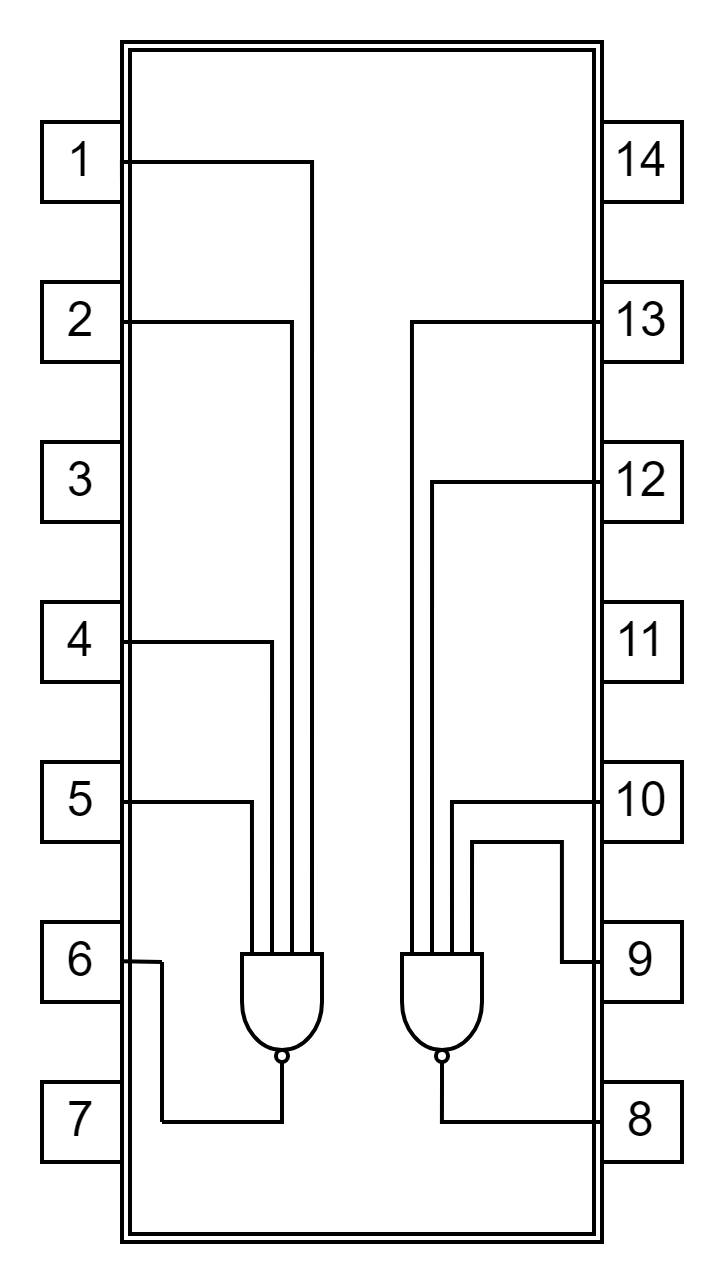
\includegraphics[width=0.3\textwidth]{7420_SCHEMA.png}
    \caption{Getekende logische schakeling van de 7420 IC. Hierbij is pin-14 de $V_{cc}$ aansluiting en is pin-7 de $GND$ aansluiting. Ook is te zien dat pin-11 en pin-3 niet in gebruik zijn!}
    \label{fig:7420SCHEMA}
\end{figure}

\subsection{Sluit met behulp van de datasheet het IC op correcte wijze aan op het IC board}


\pagebreak
\subsection{Wat is de werking van de poort en stel de bijbehorende waarheidstabel op}
De werking van de NAND-poort in de 7420 IC is als volgt: \\
Als alle vier de inputs aan staan (HIGH), dan is de output LOW. De NAND-poort geeft als output HIGH voor de rest van de mogelijke instanties.

Zie hieronder de bijbehorende waarheidstabel van de vier-input NAND-gate:
\begin{displaymath}
    \begin{array}{|c|c|c|c||c|}
    A & B & C & D & X \\ % Use & to separate the columns
    \hline % Put a horizontal line between the table header and the rest.
    1 & 1 & 1 & 1 & 0 \\
    1 & 1 & 1 & 0 & 1 \\
    1 & 1 & 0 & 1 & 1 \\
    1 & 1 & 0 & 0 & 1 \\
    1 & 0 & 1 & 1 & 1 \\
    1 & 0 & 1 & 0 & 1 \\
    1 & 0 & 0 & 1 & 1 \\
    1 & 0 & 0 & 0 & 1 \\
    0 & 1 & 1 & 1 & 1 \\
    0 & 1 & 1 & 0 & 1 \\
    0 & 1 & 0 & 1 & 1 \\
    0 & 1 & 0 & 0 & 1 \\
    0 & 0 & 1 & 1 & 1 \\
    0 & 0 & 1 & 0 & 1 \\
    0 & 0 & 0 & 1 & 1 \\
    0 & 0 & 0 & 0 & 1   
    \end{array}
    \end{displaymath}
\pagebreak
\section{De 7410}
In deze derde opdracht moesten we de 7410 IC onderzoeken en de bijbehorende opdrachten beantwoorden:

\begin{enumerate}
    \item Bepaal aan de hand van de datasheet welke type poort de 7410 bevat;
    \item Sluit met behulp van de datasheet het IC op correcte wijze aan op het IC board;
    \item Ga de werking van deze poort na;
    \item Stel de bijbehorende waarheidstabel op;
    \item Controleer hoe de uitgang van de poort zich gedraagt, indien één van de ingangen wordt opengelaten. 
\end{enumerate}
\subsection{Bepaal aan de hand van de datasheet welke type poort de 7410 bevat}
Volgens de datasheet van de 7410 IC bevat deze IC veertien pinnen in totaal waarvan pin-14 de $V_{cc}$ ingang is en pin-7 de $GND$ uitgang is. 
Daarnaast bevat deze IC drie keer drie-ingangs NAND-poorten. Zie hieronder de getekende logische schakeling:
\begin{figure}[h]
    \centering
    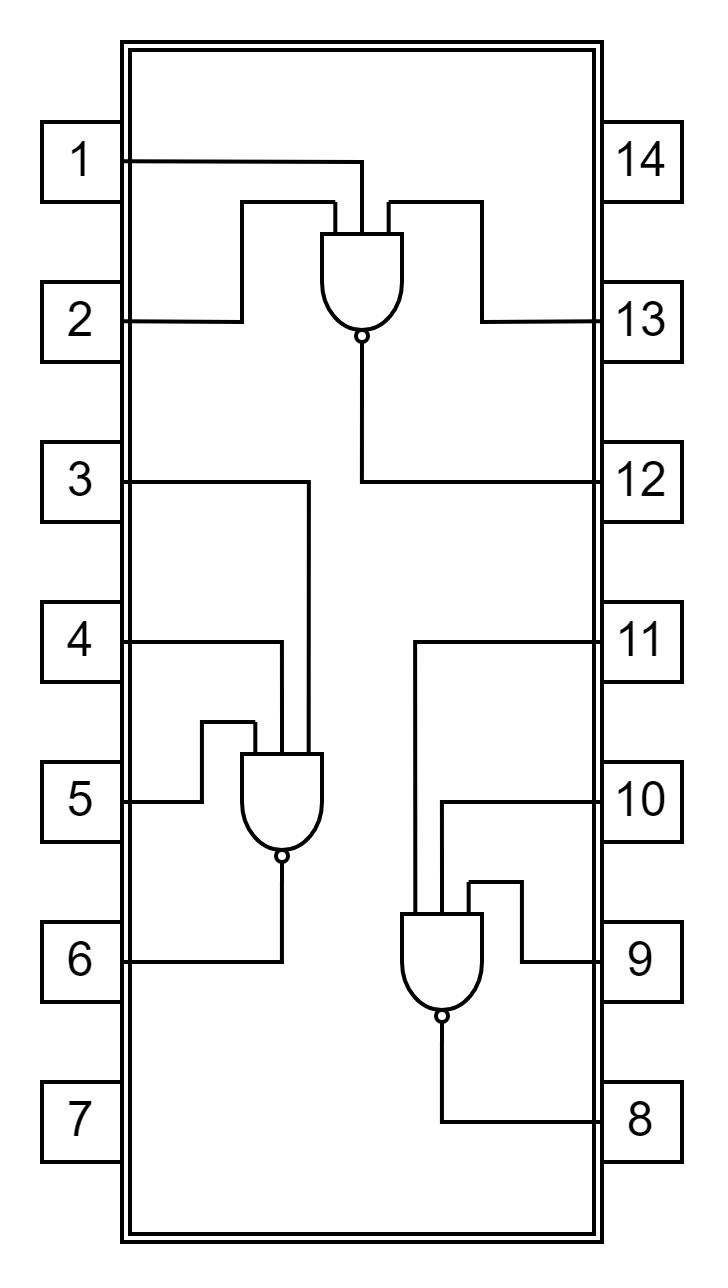
\includegraphics[width=0.3\textwidth]{7410_SCHEMA.png}
    \caption{Getekende logische schakeling van de 7410 IC. Hierbij is pin-14 de $V_{cc}$ aansluiting en is pin-7 de $GND$ aansluiting.}
    \label{fig:7410SCHEMA}
\end{figure}

\subsection{Sluit met behulp van de datasheet het IC op correcte wijze aan op het IC board}

\subsection{Ga de werking van deze poort na en stel de bijbehorende waarheidstabel op}
Deze NAND-poort bevat drie ingangen en één uitgang. Als alle drie de ingangen actief hoog (HIGH) staan, dan is de output LOW. 
Alle andere mogelijke instanties met de ingangen zullen als output HIGH geven, aangezien de output alleen LOW wordt als alle ingangen HIGH zijn. 

Zie hieronder de waarheidstabel voor de drie-ingangs NAND-poort:
\begin{displaymath}
    \begin{array}{|c|c|c||c|}
    A & B & C & X \\ % Use & to separate the columns
    \hline % Put a horizontal line between the table header and the rest.
    1 & 1 & 1 & 0 \\
    1 & 1 & 0 & 1 \\
    1 & 0 & 1 & 1 \\
    1 & 0 & 0 & 1 \\
    0 & 1 & 1 & 1 \\
    0 & 1 & 0 & 1 \\
    0 & 0 & 1 & 1 \\
    0 & 0 & 0 & 1
    \end{array}
    \end{displaymath}
\subsection{Controleer hoe de uitgang van de poort zich gedraagt, indien één van de ingangen wordt opengelaten}
Als er een poort als ingang weg wordt gelaten, dan gedraagt de NAND-poort zich als een twee-inputs NAND-poort in plaats van drie-inputs NAND-poort.
\pagebreak

\section{NAND-poort}
In deze vierde opdracht moest het gedrag van de NAND-poort onderzocht worden en daarbij moesten er ook deelopdrachten gemaakt worden, namelijk:
\begin{enumerate}
    \item Onderzoek het gedrag van de schakeling in figuur 8 door deze op te bouwen op het digiboard;
    \item Stel de bijbehorende waarheidstabel op;
    \item Stel de logische functie (Booleaanse expressie) van X op.
\end{enumerate}

\subsection{Onderzoek het gedrag van de schakeling in figuur 8 door deze op te bouwen op het digiboard}
Het gedrag van de logische schakeling is dat A en B in eerste instantie worden geïnverteerd. Dit komt, omdat beide ingangen van de NAND-poort zijn aangesloten aan A (wat ook geldt voor B en zijn NAND-poort). 
Daarna gaan $\overline{A}$ en $\overline{B}$ samen in een NAND-poort. Hierbij ontstaat er een dubbele negatie voor zowel A en B en zal de negatie verdwijnen. De AND zal veranderen in een OR, omdat de AND ook geïnverteerd wordt (wet van Morgan).
\begin{figure}[h]
    \centering
    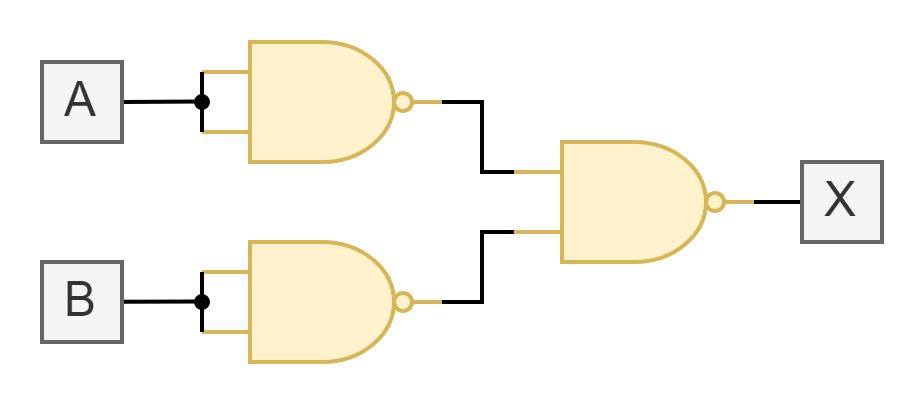
\includegraphics[width=0.5\textwidth]{figuur11.png}
    \caption{De logische schakeling van de NAND-poort opdracht.}
    \label{fig:11}
\end{figure}
\subsection{Stel de bijbehorende waarheidstabel op}
Zie de bijbehorende waarheidstabel hieronder uitgewerkt:
\begin{displaymath}
    \begin{array}{|c|c||c|c|c|}
    A & B & \overline{A} & \overline{B} & \overline{\overline{A} \cdot \overline{B}} \\ 
    \hline 
    1 & 1 & 0 & 0 & 1 \\
    1 & 0 & 0 & 1 & 1 \\
    0 & 1 & 1 & 0 & 1 \\
    0 & 0 & 1 & 1 & 0
    \end{array}
    \end{displaymath}

\subsection{Stel de logische functie (Booleaanse expressie) van X op}
De logische functie is op te stellen door gebruik te maken van de getekende logische schakeling of door de waarheidstabel af te lezen. 
In dit geval is er gekozen om gebruik te maken van de waarheidstabel: $X = \overline{\overline{A} \cdot \overline{B}}$. 
Daarnaast is de bovenstaande Booleaanse expressie te vereenvoudigen met behulp van de wet van Morgan:\\
$\overline{\overline{A} \cdot \overline{B}} \equiv A + B$. Logische functie is dan: $X = A + B$.
\pagebreak
\section{OR/NOR-poort}
In deze vijfde opdracht is het gedrag van zowel de OR-poort als de NOR-poort onderzocht. Hierbij horen er natuurlijk ook deelopdracht bij, namelijk:
\begin{enumerate}
    \item Ga de werking na van een OR-poort met twee ingangen. Stel de bijbehorende waarheidstabel op; 
    \item Controleer hoe de uitgang van een OR-poort zich gedraagt bij een open ingang;
    \item Ontwerp een NOR-poort met behulp van basispoorten;
    \item Bouw deze schakeling op het digiboard;
    \item Ga de werking van deze schakeling na;
    \item Stel de bijbehorende waarheidstabel op.
\end{enumerate}

\subsection{Ga de werking na van een OR-poort met twee ingangen. Stel de bijbehorende waarheidstabel op}
De OR-port werkt net als een plus-operatie. Dit houdt in dat als minimaal een van de twee inputs HIGH zijn, dat de output ook HIGH is. Als er geen een input HIGH is, dan is de output LOW. 
Zie de waarheidstabel en logische getekende schema hieronder:
\begin{displaymath}
    \begin{array}{|c|c||c|}
    A & B & X \\ 
    \hline 
    1 & 1 & 1 \\
    1 & 0 & 1 \\
    0 & 1 & 1 \\
    0 & 0 & 0
    \end{array}
\end{displaymath}
\begin{figure}[h]
    \centering
    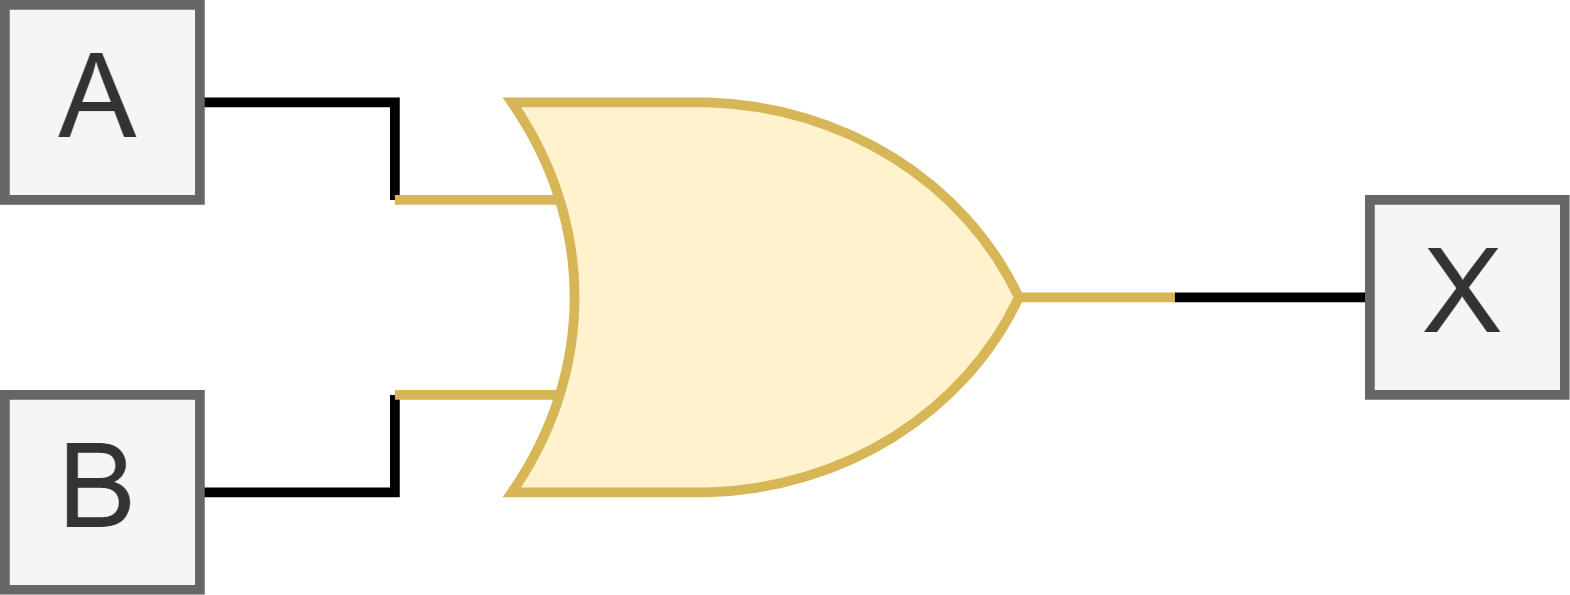
\includegraphics[width=0.5\textwidth]{OR-PORT.png}
    \caption{De logische schakeling van de OR-poort.}
    \label{fig:OR-PORT}
\end{figure}
\subsection{Controleer hoe de uitgang van een OR-poort zich gedraagt bij een open ingang}
Als er een ingang open wordt gelaten dan gedraagt de OR-poort zich als een doorgetrokken draad. Dus als je ingang A HIGH maakt, dan is de output ook HIGH, hetzelfde principe geldt ook voor LOW signalen. 
\subsection{Ontwerp een NOR-poort met behulp van basispoorten}
Ze de afbeelding hieronder:
\begin{figure}[h]
    \centering
    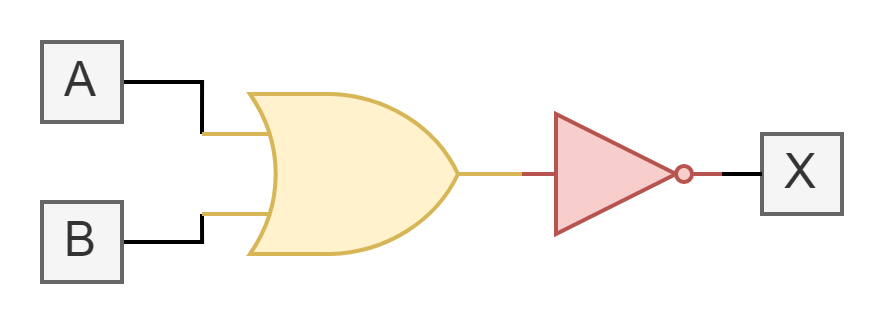
\includegraphics[width=0.5\textwidth]{NOR-PORT-BASISport.png}
    \caption{De logische schakeling van de NOR-poort gebouwd met alleen basispoorten (= NOT, AND en OR).}
    \label{fig:OR-PORT}
\end{figure}
\subsection{Bouw deze schakeling op het digiboard}
Zie de afbeelding hieronder:

lol

\subsection{Ga de werking van deze schakeling na}
De OR-poort heeft twee inputs, namelijk A en B. De OR werkt als een plus-operatie, zoals we al eerder hebben behandeld. 
Alleen nu wordt de output van de OR-poort ook nog eens in zijn geheel geïnverteerd. In de logische expressies zou dat er zo uit zien: 
$A + B$, wordt: $\overline{A+B}$ en als we dan de wet van Morgan toepassen krijgen we: $\overline{A} \cdot \overline{B}$.

\subsection{Stel de bijbehorende waarheidstabel op}
\begin{displaymath}
    \begin{array}{|c|c||c|c|c|c|}
    A & B & \overline{A} & \overline{B} & $A + B$ & \overline{A} \cdot \overline{B} \\ 
    \hline 
    1 & 1 & 0 & 0 & 1 & 0 \\
    1 & 0 & 0 & 1 & 1 & 0 \\
    0 & 1 & 1 & 0 & 1 & 0 \\
    0 & 0 & 1 & 1 & 0 & 1
    \end{array}
\end{displaymath}

\section{Conclusie}
\label{Conclusie}
In dit verslag is er onderzoek gedaan naar twee onderzoeksvragen: 
\begin{enumerate}
    \item \textit{``Hoe berekenen we de tijdconstante van een RC schakeling?''}
    \item \textit{``Hoe berekenen we de kantelfrequentie en de overdracht van een RC filter?''}
\end{enumerate}
In de inleiding zijn er doelstellingen geformuleerd die gericht zijn op het berekenen van de tijdconstante, het bepalen van het type filter, het berekenen van de kantelfrequentie en overdracht van een RC filter en het verkrijgen van de bijbehorende meetgegevens op een juiste wijze. 

Bij de eerste opdracht moesten we een RC-schakeling opbouwen waarbij de weerstand en de condensator in serie waren. Om de RC-tijd te kunnen bepalen hebben we gebruik gemaakt van een oscilloscoop. 
De RC-tijd hebben we berekend met de volgende formule: \(\tau = R*C\). De RC-tijd wordt bereikt op 63,21\% van de lading van de condensator. 
Ook hebben we onderzocht hoe we de RC-tijd kunnen halveren. Daarnaast moesten we ook verklaren waarom er meetafwijkingen waren. 

In opdracht 2 moesten we weer een RC-schakeling opzetten, alleen dan met een $V_{bron}$ van 5V AC in plaats van 12V DC. Om deze ``Alternating Current'' (wisselspanning) te krijgen, moesten we een patroongenerator gebruiken. 
De patroongenerator genereert een sinusfunctie die we nodig hebben in zowel opdracht 2 als opdracht 3. Verder moesten we de overdracht ($\frac{V_{out}}{V_{in}}$) berekenen voor 1kHz, 5kHz en 10kHz frequenties. 
Dit deden we door de volgende formule te gebruiken: $H(f)=\frac{V_{out}}{V_{in}} = \frac{1}{\sqrt{1+(2\pi RC f)^2}}$. Daarnaast moesten we zowel in opdracht 1 als in opdracht 2 de frequentieresponse tekenen, en daarvoor moesten we eerst de kantelfrequentie berekenen. 
De kantelfrequentie hebben we berekent met: $f_k=\frac{1}{2\pi RC}$. Op de punt van de kantelfrequentie bevindt zich het -3dB punt, wat belangrijk is voor het plotten van de grafiek. 
Tenslotte moesten we nog nagaan of de theoretische berekende overdrachten wel klopten. Dit hebben we gedaan door alle drie de $V_{out}$ (van de verschillende frequenties) af te lezen van de oscilloscoop, want door de $V_{out}$ te delen door de $V_{in}$ kun je ook de overdracht bepalen. 

Tenslotte in opdracht 3 moesten we de schakeling van opdracht 2 kopiëren, alleen moesten nu de condensator en weerstand van hun plek omgewisseld worden. 
We gingen dezelfde vragen beantwoorden als die van in opdracht 2. Toen zagen we al snel dat het verwisselen van componenten ervoor zorgde dat alles omgekeerd ging werken. 
In opdracht 2 hebben we gezien dat we te maken hadden met een laagdoorlaatfilter, want hoe lager de frequenties waren, des te groter de overdracht werd. 
In opdracht 3 was dit effect net andersom. We constateerde dit al snel bij de berekeningen, want daar zagen we ook dat des te hoger de frequenties waren, des te groter de overdracht werd en bij lage frequenties was de overdracht juist heel klein. 
Deze type filter wordt dan ook wel de hoogdoorlaatfilter genoemd, omdat deze filter alleen hoge frequenties doorlaat. De overdracht van een hoogdoorlaatfilter kan op de volgende manier berekend worden: $H(f)=\frac{2\pi RCf}{\sqrt{1+(2\pi RC f)^2}}$. 
Ook moest de kantelfrequentie opnieuw berekend worden. Dit werd op dezelfde manier gedaan als in opdracht 2: $f_k=\frac{1}{2\pi RC}$, dus met de kantelfrequentie kunnen we bepalen waar het -3dB punt zit van de filter en daarmee kunnen we ook een frequentieresponse maken. 

De in de inleiding geformuleerde doelstellingen zijn met behulp van de 3 opdrachten succesvol behaald. We hebben met behulp van deze opdrachten eigenschappen van individuele componenten en reactie op verwisselen posities kunnen waarnemen en verklaren.


\pagebreak






\nocite{*}
\section{Bronvermelding}

\bibliography{library.bib}
\bibliographystyle{IEEEtran}

\pagebreak
\end{document}